\chapter{Il progetto}
\fancyhead[RO]{\bfseries Il progetto}

L'obiettivo del progetto è quello di offrire un'interfaccia uomo-macchina, che permetta all'utente di interagire con la telecamera virtuale della scena, utilizzando il proprio volto come controller. Utilizzando la tecnica dell'head-tracking viene rilevato il volto, il  movimento del quale determina la trasformazione della prospettiva con cui è visualizzata la scena, generando l'illusione della presenza di profondità al di là dello schermo. Con un rilevamento efficiente del volto, e con una scena ben fatta, è possibile creare una visione tridimensionale senza l'uso di occhialini 3D.

L'applicazione è stata sviluppata in due versioni, utilizzando due API differenti: OpenGL e Ogre3D.

La prima versione è il risultato dello studio di fattibilità e può essere considerato un prototipo.
Utilizzare OpenGL, il quale lavora a basso livello, è stato utile per comprendere meglio il comportamento del sistema in base alle trasformazioni adottate. La scena creata rappresenta l'interno di una scatola, con la parte frontale aperta posizionata sul near plane, in modo da dare l'illusione che lo stesso schermo del PC sia l'apertura della stessa; all'interno sono stati aggiunti dei semplici cubi.

La seconda versione è stata sviluppata una volta compresi i principi delle trasformazioni adottate. L'utilizzo di Ogre3D ha portato a dei miglioramenti in termini di grafica, grazie alla possibilità di importare facilmente scene create tramite altri software di modellazione. Visto che questa versione presenta anche dei miglioramenti in termini di efficienza, la prenderemo in esame ed analizzeremo il suo codice, trattando le fasi principali in dettaglio.
In seguito sarà dedicata una sezione all'importazione delle scene in Ogre.


L'applicazione è stata scritta in C++ ed è divisa in due parti principali:
\begin{itemize}
\item Un modulo OpenCV separato da tutto il resto, che offre un metodo che fornisce le coordinate del volto rilevate nel momento in cui viene richiamato.
\item La parte grafica sviluppata usando Ogre3D.
\end{itemize}


\section{Il funzionamento dell'applicazione}
Il cuore dell'applicazione risiede nelle trasformazioni da applicare alla scena. In ogni frame sono eseguite diverse fasi, a partire dall'ottenimento delle coordinate del volto, arrivando a trasformare la prospettiva nel modo voluto. Vediamo in breve le fasi:
\begin{enumerate}
\item Ottenimento delle coordinate del volto, in pixel (relative alla webcam).
\item Applicazione di un filtro per eliminare il rumore generato a causa dell'imprecisione del rilevamento.
\item Trasformazione delle coordinate in punti dello spazio 3D.
\item Calcolo dei sei piani del frustum in base alle coordinate dell'osservatore, e creazione della projection matrix.
\item Calcolo dei vettori necessari per la view matrix, e creazione della stessa.
\item Creazione di una matrice di traslazione per aggiustare lo spostamento della telecamera, in modo che l'apertura della scena sia fissata ai bordi dello schermo.
\item La matrice relativa alla trasformazione finale della telecamera è data dal prodotto delle tre matrici calcolate nei tre passi precedenti.
\end{enumerate}
Analizzando in dettaglio le varie fasi:

\subsection*{Step 1: Ottenimento delle coordinate}

Grazie al modulo OpenCV, richiamando una semplice funzione possiamo ottenere le coordinate del volto in un dato frame.\\

Di seguito un estratto di codice della funzione nel modulo OpenCV.

\begin{lstlisting}
bool getFaceCoord(int* x, int* y, int* z ) {
...

  if ( detectAndDisplay( pt, z ) ) {
        *x = pt.x;
        *y = pt.y;
        *z = z;
        return true;
    } 
    return false;
}
...

bool detectAndDisplay( cv::Point& center, int& z ) {
...
face_cascade->detectMultiScale( frame_gray, faces, 1.1, 3,
                                0|cv::CASCADE_SCALE_IMAGE, 
                                cv::Size(90,110) );
    
    // se viene rilevato un solo volto
    if (faces.size() == 1 ) { 
            center.x = faces[0].x + faces[0].width*0.5;
            center.y = faces[0].y + faces[0].height*0.1;
            z = faces[0].width;
    }
    return true;
}
\end{lstlisting}
\texttt{detectMultiscale} è un metodo della classe \textit{CascadeClassifier}; il cascade utilizzato è \texttt{haarcascade\_frontalface\_default.xml}, fornito da OpenCV, il quale contiene le informazioni per rilevare volti umani. Il metodo perciò rileva i volti e inserisce i risultati in un vettore di matrici, \textit{faces}. Va controllata la dimensione del vettore \textit{faces}, in quanto il volto rilevato deve essere uno solo, per evitare di generare confusione tra le coordinate.

Successivamente si memorizzano le tre coordinate del volto:
\begin{itemize}

\item Per la $x$ si considera la coordinata $x$ del centro del volto rilevato.
\item Per la $y$ si considera la coordinata $y$ a $1/10$ dell'altezza del volto, partendo dall'alto. Con varie prove si è notato che gli occhi sono rilevati all'incirca a questa altezza.
\item Per la $z$ si considera la larghezza del volto in pixel. Purtroppo non è stato trovato un modo migliore per stimare la distanza dallo schermo, perciò ci si è accontentati di questa misurazione abbastanza grossolana.  
\end{itemize}


In seguito il codice presente nella parte Ogre3D, in cui viene richiamata la funzione descritta in precedenza:
\begin{lstlisting}
Ogre::Real x,y,z;
int coordX = 0 ,coordY = 0,coordZ = 0;
if (!getFaceCoord( &coordX, &coordY, &coordZ ) ) {
    x = flX->interpolate(prevX);
    y = flY->interpolate(prevY);
    z = flZ->interpolate(prevZ);
}
\end{lstlisting}
Il metodo \texttt{getFaceCoord()} viene richiamato passando come parametri tre interi. Se la funzione ritorna true si continua con le fasi successive, altrimenti significa che c'è stato un errore nel frame corrente e perciò vengono prese in considerazione le coordinate del frame precedente, per evitare crash o blocchi nell'applicazione.

\subsection*{Step 2: Filtro antirumore}
Come abbiamo detto nel paragrafo relativo ad OpenCV, vari fattori creano difficoltà nel tracking; fra le varie conseguenze, una è la generazione di una sorta di rumore: rimanendo fermi, le coordinate rilevate oscillano sempre di minimo 2 o 3 pixel, e questo determina un fastidioso tremolio nella scena.

Per ovviare (almeno in parte) a questi problemi, è stato creato un piccolo algoritmo che filtra il rumore generato dal rilevamento, cercando di preservare la fluidità nei movimenti. Di seguito la funzione che elimina il rumore di fondo.
\begin{lstlisting}
void Filter::filter(Ogre::Vector2 &cVec, int erMin) {
    int coord = cVec.x; //coordinata attuale
    int p     = cVec.y; //coordinata precedente
	
    // se coord = 0 il rilevamento non e' avvenuto
    // percio' si considera la coordinata precedente
    if (coord == 0) {
        cVec.x = p;
        return;
    }
    
    int dif = abs( coord - p );
    
    // se e' sotto la soglia minima salva 
    // la coordinata precedente
    if ( dif <= erMin ) {
        cVec.x = p;     	
    }
    // altrimenti pone la precedente uguale all'attuale
    else {
        cVec.y = coord;	
    }  
}
\end{lstlisting} 

La funzione prende in input un vettore con la coordinata attuale e precedente, e una soglia minima di errore.
Se la differenza in valore assoluto tra le due coordinate è minore della soglia minima, allora si scarta la nuova coordinata e si utilizza la precedente, perciò non viene generato movimento. Questo elimina il rumore, ma crea un altro problema: quando l'utente si sposta normalmente la prospettiva viene trasformata eseguendo movimenti a scatti, dovuti proprio al filtro che elimina comunque dati utili.

Per risolvere questo secondo problema è stato creato un secondo algoritmo che interpola i movimenti, rendendoli più fluidi grazie alla generazione di coordinate intermedie tra l'attuale e la precedente. Analizziamo il codice.
\begin{lstlisting}
Ogre::Real FluidFilter::interpolate(Ogre::Real c) {
    // se la coordinata rilevata e' la stessa
    // si avvicina ad essa
    if ( lastCoord == c ) {

        if (count == 1) {
            count--;
            last = c;
        }
        else if ( count > 0) {
            count--;
            last += gap;
        }
    }
    
    // altrimenti ricalcola il gap
    else {
        lastCoord = c;
        count = n;
        gap   =  ( c - last ) / n ;
        last += gap;
    }
    
    return last;
}
\end{lstlisting} 
La classe \textit{FluidFilter} contiene, fra gli attributi, un contatore e la coordinata interpolata nel frame precedente. Il contatore diminuisce quando le coordinate non cambiano, in modo da rendere l'interpolazione finita. Se le coordinate cambiano, si calcola un gap dato dalla differenza tra quella attuale e quella interpolata precedentemente, diviso per n; n influisce sulla qualità dell'interpolazione: all'aumento di n i movimenti sono più fluidi, ma, come effetto contrario, sono più rallentati. Con un valore di n pari a 3 o 4 l'effetto finale è accettabile, rendendo il delay quasi impercettibile e preservando una buona fluidità.

\subsection*{Step 3: Trasformazione delle coordinate}
Il sistema di coordinate di OpenCV è differente da quello relativo alla scena. Innanzitutto le coordinate fornite da OpenCV sono di tipo intero e dipendono dalla risoluzione della webcam: per esempio, con una risoluzione $640\times 480$, la $x$ può oscillare tra $0$ e $640$ e la $y$ tra $0$ e $480$; inoltre l'origine è situato nell'angolo in alto a sinistra della finestra. Il sistema del mondo 3D utilizza coordinate di tipo Real e l'origine si trova nel punto $(0,0,0)$. Per rendere compatibili i due sistemi deve essere applicata una conversione.

Con qualche prova di calibrazione si è infine deciso di utilizzare i seguenti calcoli per convertire le coordinate (già filtrate):
\begin{lstlisting}
    z = z / 150.0f;
    x = -( ( ( x - xCam/2 ) / 15.0f ) / (xr*ar) );
    y = -( ( ( y - yCam/2 ) / 15.0f ) / (yr*ar) );  
\end{lstlisting}  

\textit{xCam} e \textit{yCam} rappresentano le dimensioni della webcam in pixel. La prima sottrazione nella $x$ e nella $y$ trasla l'origine relativo ad OpenCV nell'orgine relativo al mondo virtuale.\\
\textit{ar} è il reciproco dell'aspect ratio della finestra aperta.\\
\textit{xr} e \textit{yr} sono rispettivamente il rapporto delle dimensioni della finestra per quelle della webcam, sempre in pixel. La divisione finale dovrebbe permettere di mantenere una proporzionalità dei movimenti utilizzando risoluzioni diverse. Per una maggiore efficienza, le coordinate dovrebbero essere calcolate anche in funzione della distanza dalla telecamera; purtroppo però questo studio è risultato troppo complesso, quindi è stato tralasciato.

\subsection*{Step 4: Projection matrix}
Una volta calcolate le coordinate effettive, queste vengono memorizzate nel vettore \textit{face}.
Tramite il vettore \textit{face}, si ricalcolano i piani del frustum nel seguente modo:
\begin{lstlisting}
    n = -face.z + nP;     //near plane
    f = n + sceneLength;  //far plane
    r = width - face.x;   //right plane
    l = r - 2*width;      //left plane
    t = height - face.y;  //top plane
    b = t - 2*height;     //bottom plane

\end{lstlisting}

Il near plane è calcolato in base alla distanza (approssimata) dell'osservatore, in modo che, quando questo si avvicina allo schermo, si crea un effetto di allungamento della scena. Per fare un esempio dell'effetto immaginiamo di vedere una finestra da lontano; più ci avviciniamo alla finestra e più ampia diventa la visuale di ciò che c'è al di fuori. Inoltre il valore del near plane varia in base alla costante \texttt{nP}, definita dall'utente, che determina la distanza focale di default.

Il far plane dipende dal near plane e dalla profondità della scena.

Le successive quattro coordinate sono calcolate in modo da formare un rettangolo che si sposta lungo il piano XY in base alla posizione dell'utente, generando il frustum asimmetrico che permette di distorcere la prospettiva. \textit{width} e \textit{height} coincidono rispettivamente con la metà della larghezza e dell'altezza della scena. Come vedremo in seguito, queste dimensioni dovrebbero essere uguali a quelle della scena ed inoltre dovrebbero rispettare l'aspect ratio della finestra aperta.

Successivamente viene richiamata una funzione che prende in input le sei coordinate e calcola la matrice di proiezione\footnote{La matrice di proiezione vista nella sezione 2.2.2}, restituendola:

\begin{lstlisting}
Ogre::Matrix4 frustum = Ogre::Matrix4(
        
        2*n/(r-l),         0, (l+r)/(r-l),           0,
                0, 2*n/(t-b), (t+b)/(t-b),           0,
                0,         0,     f/(n-f), (n*f)/(n-f),
                0,         0,          -1,           0
);

\end{lstlisting}

\subsection*{Step 5: View matrix}
Per costruire la view matrix occorrono tre vettori. I primi due sono calcolati così:
\vspace{1cm}
\begin{lstlisting}
eye    = Ogre::Vector3(-face.x, -face.y, -face.z);

target = Ogre::Vector3(r - width, t - height, -n);
\end{lstlisting}

\textit{eye} utilizza le coordinate del volto, con il segno opposto. Quando il frustum viene spostato lungo una direzione, l'effetto prodotto è uno spostamento della scena nel verso opposto. Questo perchè il frustum rappresenta la porzione di spazio da visualizzare, non la scena. Ad esempio se noi stiamo guardando un oggetto e nel frattempo che ci muoviamo verso destra, dal nostro punto di vista l'oggetto si starà spostando verso sinistra. Perciò, per mantenere allineati i movimenti, il vettore \textit{eye} deve essere l'inverso di \textit{face}.
Senza questa accortezza si crea un effetto di rotazione, come è possibile vedere nella figura \ref{wrong-eye}.

\begin{figure}[htbp]
\centering
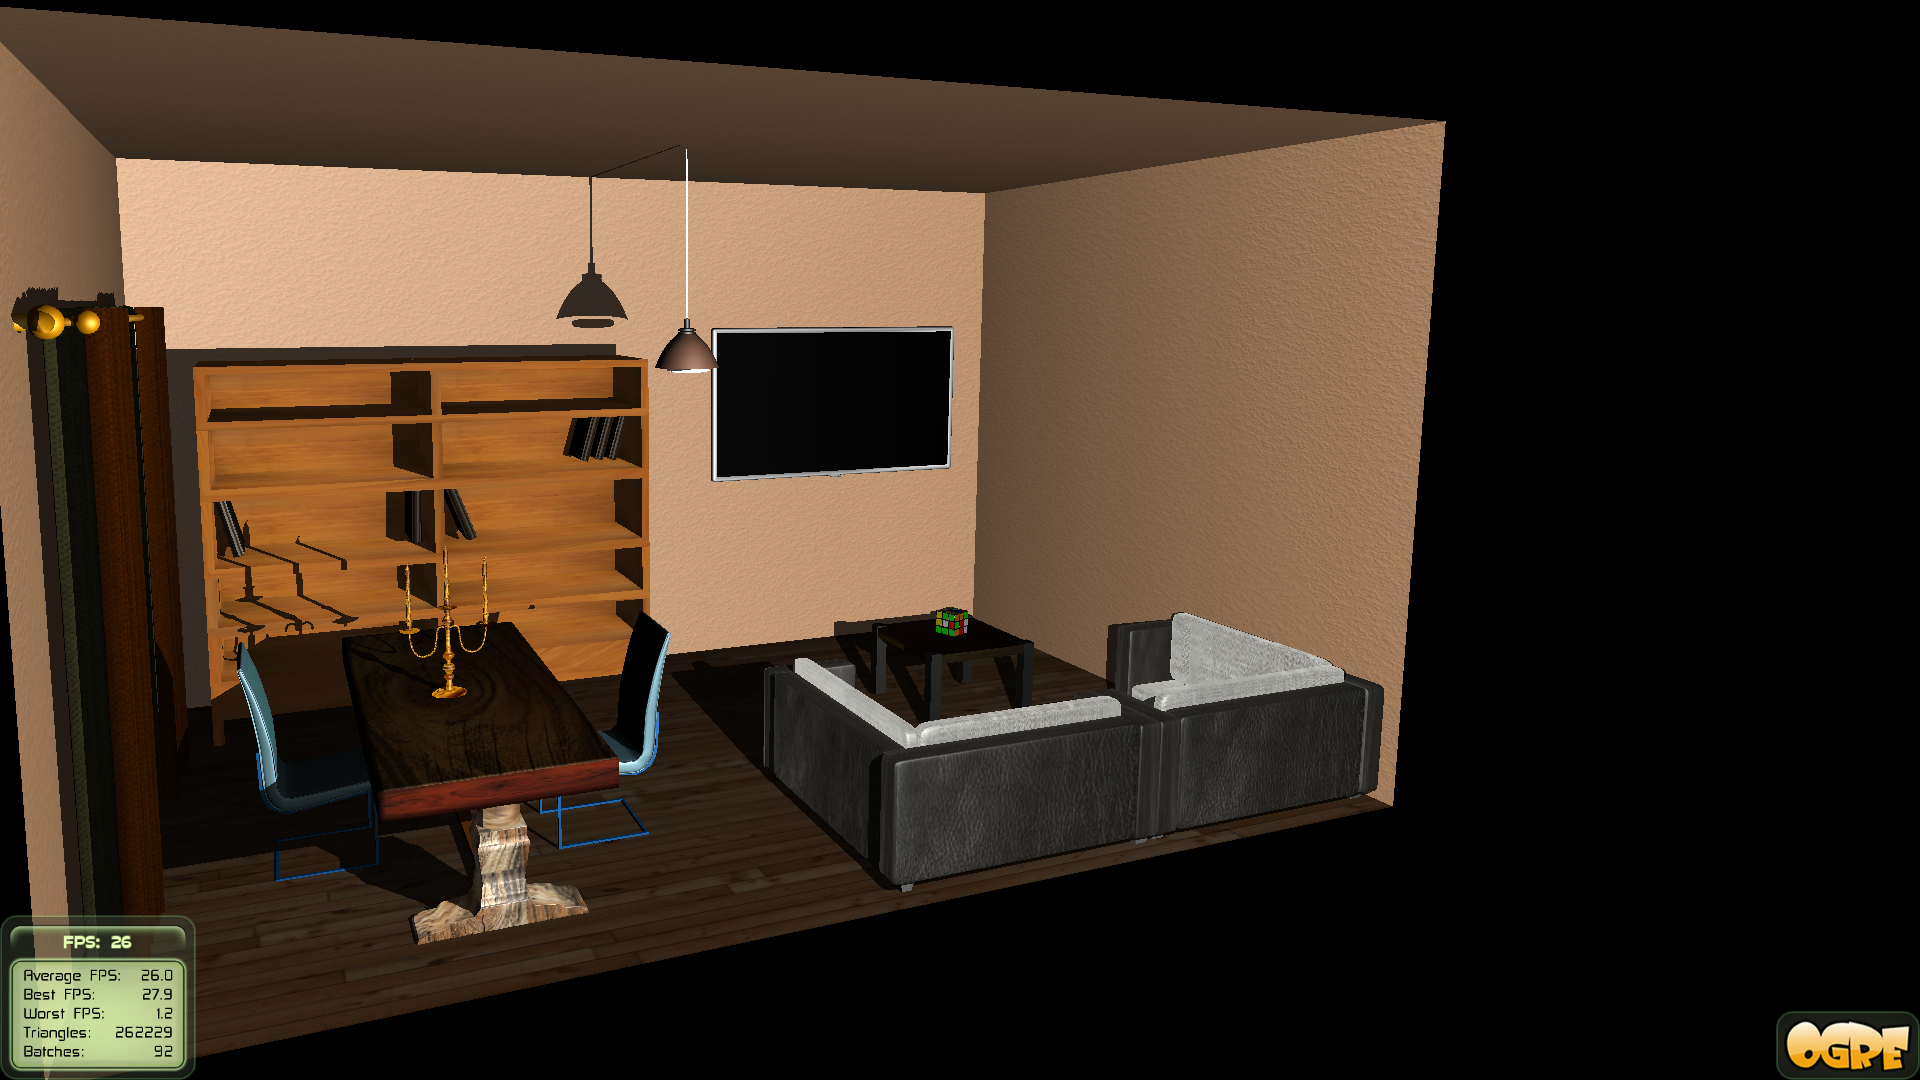
\includegraphics[width=0.7\textwidth]{images/progetto/ogre-wrong.png}
\caption{Trasformazione ottenuta calcolando in modo errato il vettore \textit{eye}.\label{wrong-eye}}
\end{figure}


\textit{target} è il centro del rettangolo che rappresenta il near plane, in quanto il punto osservato deve essere sempre il centro della scena.

In seguito viene richiamato un metodo che calcola la view matrix:

\begin{lstlisting}
Ogre::Vector3 up = Ogre::Vector3(0, 1, 0);
Ogre::Vector3 z = (eye - target); 
z.normalise();     // forward vector.
Ogre::Vector3 x = (up.crossProduct(z)); 
x.normalise();    // right vector.
Ogre::Vector3 y = z.crossProduct(x); // up vector.
 
Ogre::Matrix4 viewMatrix = Ogre::Matrix4(
    x.x, x.y, x.z, -(x.dotProduct(eye)),
    y.x, y.y, y.z, -(y.dotProduct(eye)),
    z.x, z.y, z.z, -(z.dotProduct(eye)),
      0,   0,   0,                    1
);
\end{lstlisting}
Il vettore \textit{up} equivale all'asse Y; la base ortonormale e la matrice sono calcolati come è stato visto nella sezione relativa alle trasformazioni.


\subsection*{Step 6: Traslazione} 
Grazie alle trasformazioni calcolate in precedenza, la prospettiva della telecamera virtuale viene collegata a quella dell'utente; tuttavia sono generati anche degli spostamenti indesiderati della scena, che possono farla scomparire oltre lo schermo, in quanto la telecamera virtuale in realtà sta fluttuando in base ai nostri movimenti. La figura \ref{no-transl} mostra l'effetto indesiderato.

\begin{figure}[htbp]
\centering
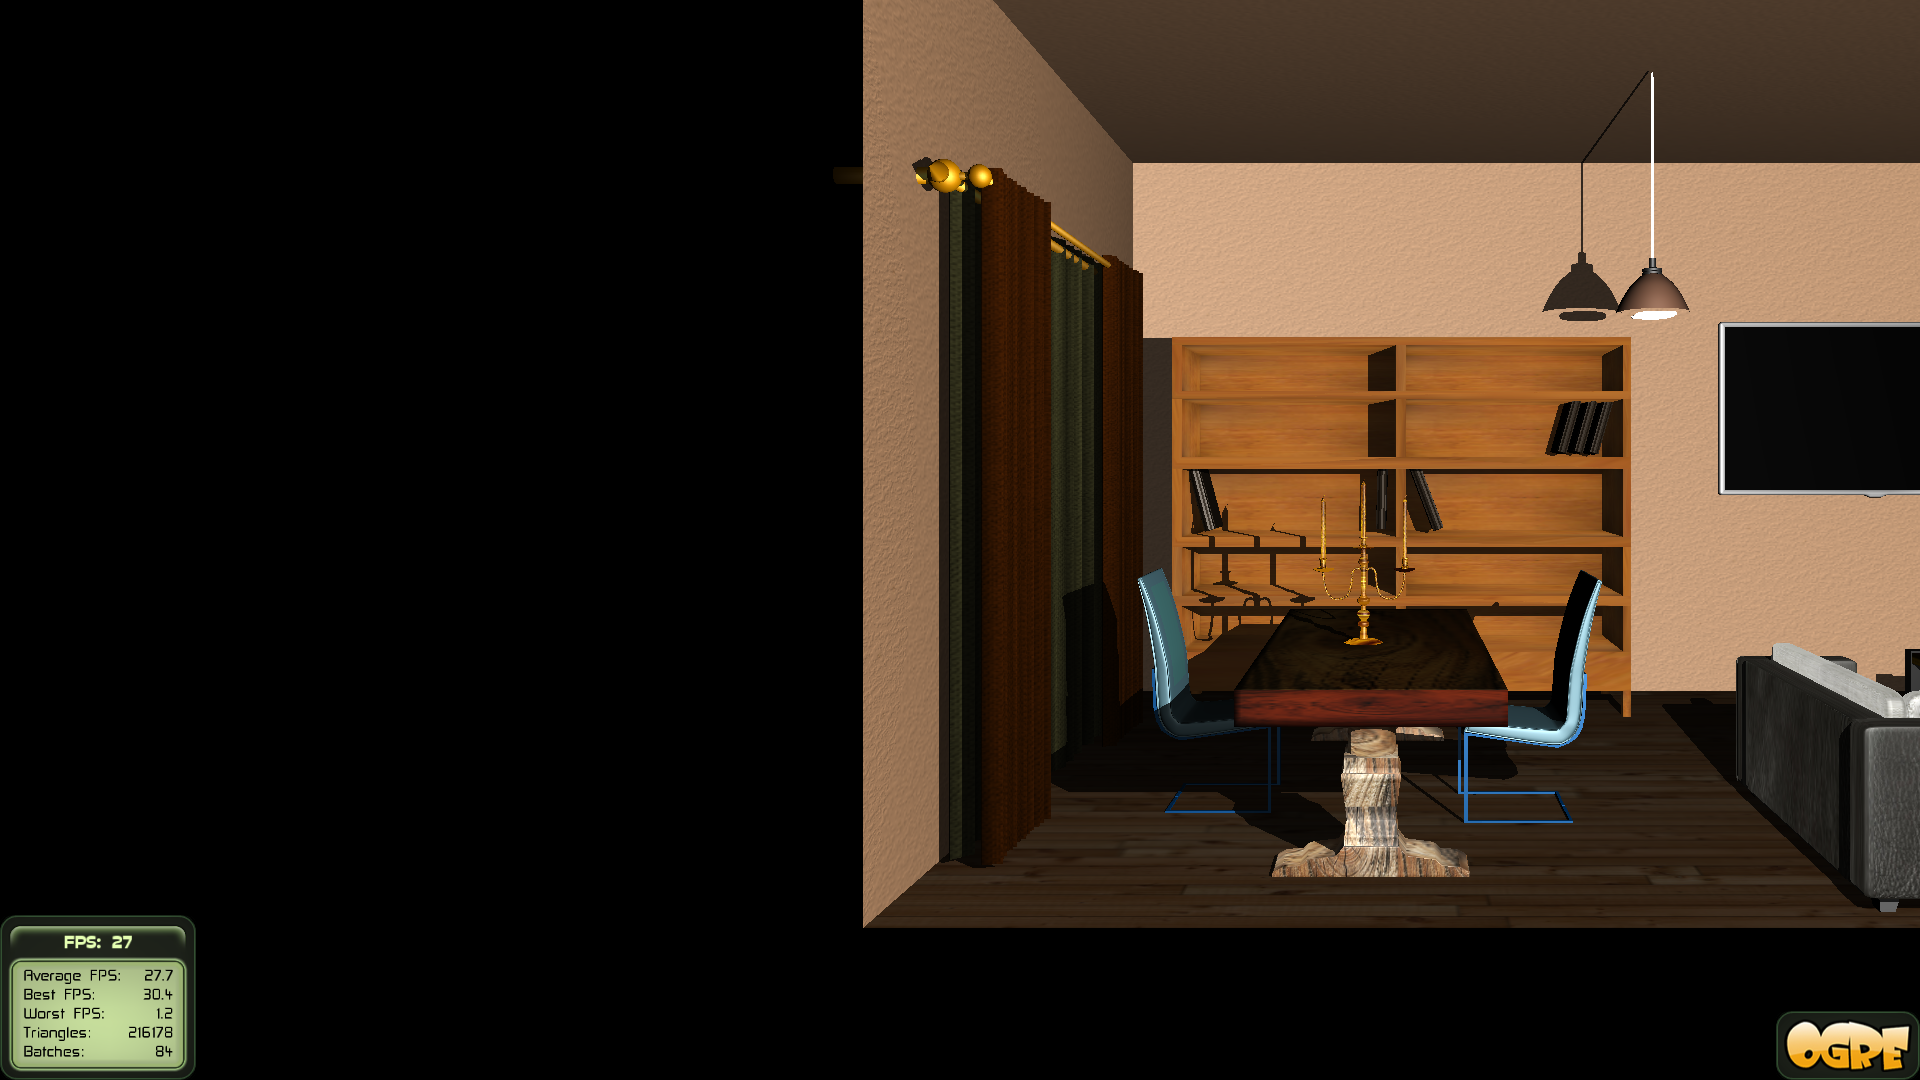
\includegraphics[width=0.7\textwidth]{images/progetto/ogre-transl.png}
\caption{Scena fluttuante, dovuta all'assenza di traslazione.\label{no-transl}}
\end{figure}
Per ottenere un corretto risultato, la scena deve rimanere ferma, cioè l'apertura della scatola deve essere fissata allo schermo; per ottenere ciò occorre una traslazione che annulli gli spostamenti generati.
\vspace{1.5cm}

\begin{lstlisting}
Ogre::Vector3 translVec = Ogre::Vector3(
            -face.x + r - width,
            -face.y + t - height,
            0
    );

Ogre::Matrix4 translMat = Ogre::Matrix4::IDENTITY;
translMat.makeTrans(translVec);
\end{lstlisting}
Si calcola il vettore \textit{translVec}, che rappresenta lo spostamento da effettuare, e poi questo viene passato come parametro al metodo \texttt{makeTrans}, il quale restituisce la matrice di traslazione desiderata.

\subsection*{Step 7: Trasformazione finale}
In OpenGL la trasformazione finale, relativa alla telecamera, è rappresentata da una matrice, che è il prodotto tra la traslazione, la matrice di proiezione e la view matrix:
\vspace{0.5cm}
\begin{lstlisting}
camera = translMat * frustum * viewMatrix;
\end{lstlisting}
In Ogre questa operazione è eseguita dal framework, perciò è sufficiente impostare le matrici calcolate, richiamando i seguenti metodi:
\begin{lstlisting}
mCamera->setCustomViewMatrix(true, translMat*viewMatrix);
mCamera->setCustomProjectionMatrix(true,frustum);
\end{lstlisting}



\section{Importazione scene}
Un'ulteriore feature dell'applicazione è quella di poter importare dall'esterno una qualsiasi scena, per poterla visualizzare in modo più interattivo.

%Un'ulteriore feature che si voleva aggiungere all'applicazione era quella di poter caricare una qualsiasi scena, modellata con diversi software, per poterla visualizzare in modo più interattivo.

\subsection{Importazione con OpenGL}
In OpenGL è stato utilizzato un parser per file con estensione .obj\footnote{File esportati da Blender, che contengono informazioni quali le coordinate dei vertici, delle normali, coordinate uv per mappare le texture, etc..}, il quale inserisce le informazioni dei modelli nei buffer utilizzati per il rendering. All'avvio del programma viene esaminata una directory apposita e, per ogni file .obj rilevato, ne viene fatto il parsing. In questo modo, per ogni modello, vengono creati diversi buffer, che saranno usati nella fase di rendering.

Purtroppo questo processo si è rivelato oneroso in OpenGL e ha portato anche ad alcune problematiche che hanno determinato la scelta di compiere questo ulteriore passo utilizzando il framework Ogre3D.

\subsection{Importazione con Ogre3D}
Esistono diversi exporter per software di modellazione quali Blender, Maya, 3D Studio Max, etc, per esportare scene e convertirle nel formato riconosciuto da Ogre. I modelli hanno estensione .mesh, mentre le informazioni relative ai materiali sono raccolte in file con estensione .material.

Per ottenere effetti più apprezzabili nelle trasformazioni, conviene che la scena rappresentata sia racchiusa da un box, con l'apertura frontale. Come esempio è stata preparata una scena in Blender, raffigurante un salotto, come si può vedere nella figura \ref{liv-room} \footnote{Alcuni modelli sono stati scaricati dal sito BlendSwap\cite{blendswap}.}.

\begin{figure}[htbp]
\centering
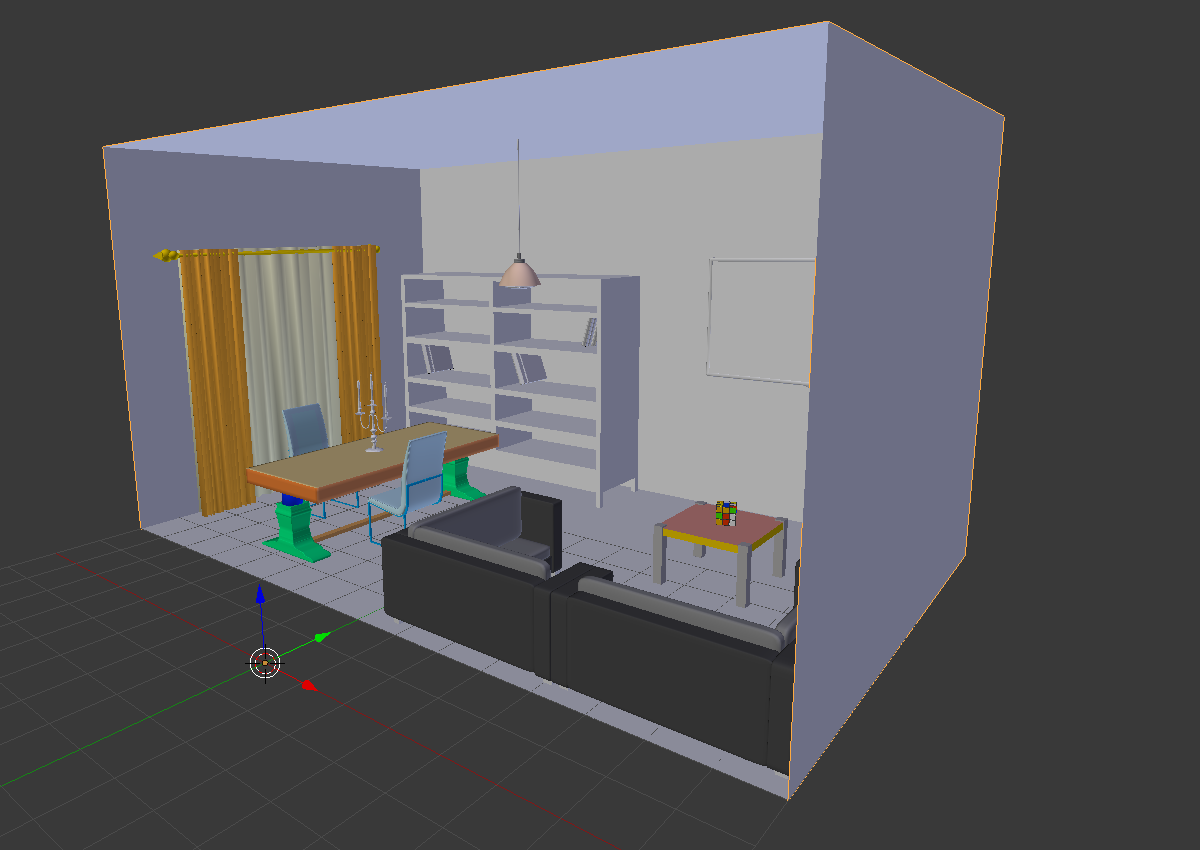
\includegraphics[width=0.7\textwidth]{images/progetto/living-room.png}
\caption{Scena modellata in Blender.\label{liv-room}}
\end{figure}

Da notare il fatto che le misure del box che racchiude la scena, in questo caso, ha un aspect ratio di $16/9$, infatti la lunghezza è pari a 16 unità mentre l'altezza è di 9 unità. Sono state scelte queste dimensioni per rispettare l'aspect ratio dello schermo. In Ogre è possibile scegliere la risoluzione della finestra all'avvio dell'applicazione, perciò si deve fare attenzione a rispettare il formato, in quanto rapporti diversi possono creare effetti di stiramento o di rimpicciolimento lungo una o entrambe le dimensioni.

Per ottenere una trasformazione corretta, il nostro frustum dovrebbe avere le stesse dimensioni della scena importata, ed inoltre il near plane andrebbe posizionato ad una distanza pari alla distanza da dove inizia la scena, in modo che il near plane coincida con l'apertura del box.

Un'ulteriore operazione da fare, all'avvio dell'applicazione, è quella di traslare la scena in modo che sia centrata nell'origine, per rientrare nella porzione di spazio considerato nel frustum.
Dopo la traslazione la scena sarà posta come è visibile nella figura \ref{transl-liv-room}. L'origine è rappresentato dai tre assi cartesiani colorati.

\begin{figure}[htbp]
\centering
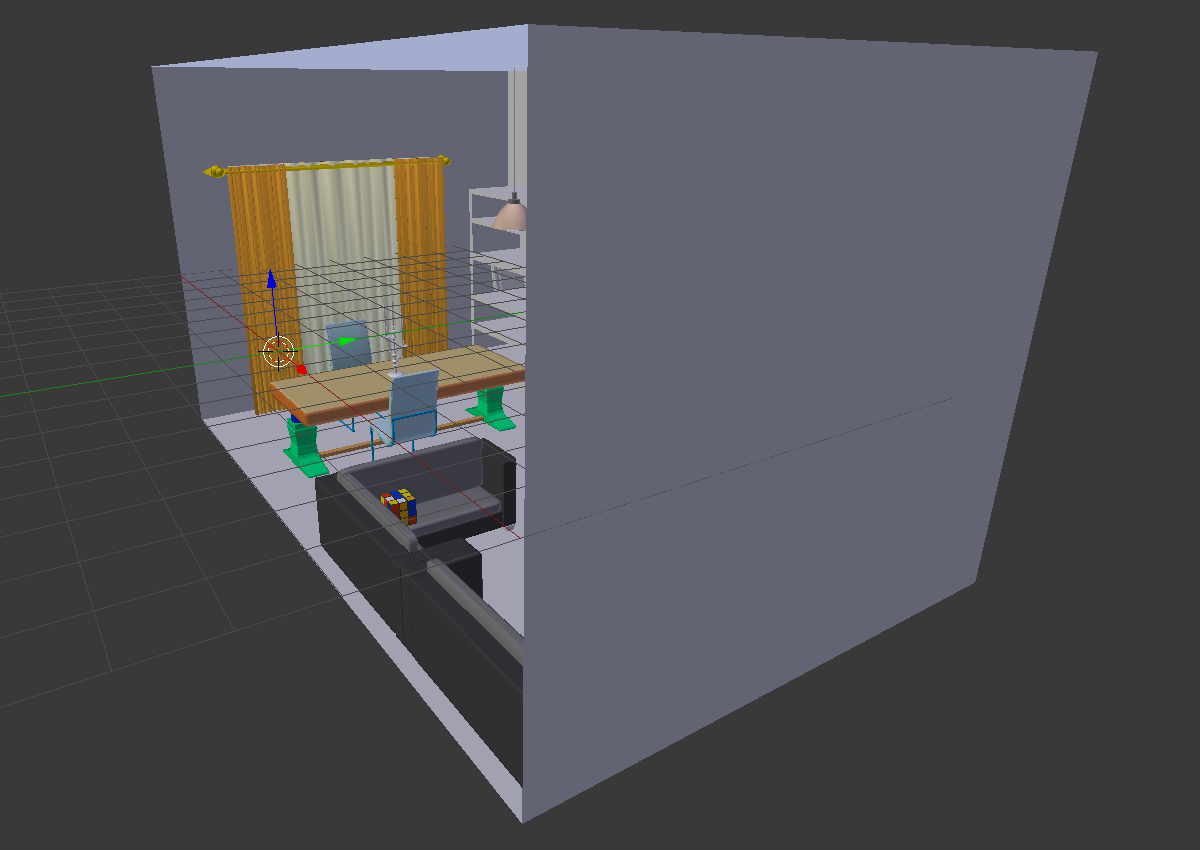
\includegraphics[width=0.7\textwidth]{images/progetto/living-room-translated.png}
\caption{La scena dopo la traslazione.\label{transl-liv-room}}
\end{figure}


Per quanto riguarda la $z$, la nostra scena inizia alla coordinata $y=2$ (l'asse Y di Blender corrisponde all'asse -Z in Ogre3D), perciò il near plane sarà posto ad una distanza pari a 2 lungo l'asse -Z, rispetto all'origine. Ovviamente il near plane è variabile, per determinare gli effetti di allontanamento o avvicinamento, ma comunque lo spostamento è corretto dalla view matrix, in modo che il near plane sia sempre coincidente con l'apertura del box.

Tutte queste condizioni sono necessarie affinché i bordi della scena siano sempre fissati ai bordi dello schermo del pc, in modo da illudere maggiormente l'occhio. Ovviamente senza questi accorgimenti la trasformazione continuerebbe comunque a funzionare in modo corretto, ma gli effetti ottenuti non garantirebbero l'illusione che l'applicazione ha lo scopo di creare.
 

